\documentclass[
	papersize=A4,
		%% e.g., "A4", "letter", "legal", "executive", ...
		%% The size of the paper of the resulting PDF file.	
	fontsize=12pt, 
	 	%% e.g., 10pt, 11pt, 12pt
	 	%% The font size of the main text in pt (points).
	laterality=oneside, 
	 	%% "oneside" or "twoside"
	 	%% Either you are creating a document which is printed on both, left pages
	 	%% and right pages (twoside) or you create a document which is printed
	 	%% on right pages only (oneside).
	draft=false,
	 	%% "true" or "false"
	 	%% Use draft mode? If true, included graphics are replaced by empty
	 	%% rectangles (of same size) and overfull boxes (in margin space) are
	 	%% marked with black box (-> easy to spot!)
	parskip=half,
	 	%% e.g., "no", "full", "half", ...
	 	%% How to separate paragraphs: indention ("no") or spacing ("half",
	 	%% "full", ...).
	BCOR=0mm,
	 	%% Inner binding correction. This value depends on the method which is
	 	%% being used to bind your printed result. Some techniques do not
	 	%% require a binding correction at all ("0mm"), other require for
	 	%% example "5mm". Refer to KOMA script documentation for a detailed
	 	%% explanation what a binding correction is and how to measure it.
	linespread=1.15,
	 	%% e.g., 1.0, 1.5, 2.0
	 	%% Line spacing in %/100. For example 1.5 means 150% of the usual line
	 	%% spacing. Please use with caution: 100% ("1.0") is fine because the
	 	%% font was designed for it.
	language={english,ngerman},
	 	%% "english,ngerman", "ngerman,english", ...
	 	%% NOTE: The *last* language is the active one!
	 	%% See babel documentation for further details.
	biblatex, % use biblatex
	% bibtex % use bibtex
		%% Choose the bibliography system you want to use, either 
		%% "biblatex" or "bibtex". Note that you also have to change the 
		%% bibfile below to reflect the correct one. 
	bibfile=99--references.bib,
	% bibfile=references-bibtex.bib,
	 	%% Name of the biblatex file that holds the references.
	biblatexstyle=alphabetic,
	% biblatexstyle=authoryear,
	 	%% BibLaTeX-settings: (see biblatex reference for further description)
	 	%% e.g., "alphabetic", "authoryear", ...
	 	%% The biblatex style which is being used for referencing. See
	 	%% biblatex documentation for further details and more values.
	 	%%
	 	%% CAUTION: if you change the style, please check for (in)compatible
	 	%%          "biblatex" package options in the file
	 	%%          "template/preamble.tex"! For example: "alphabetic" does
	 	%%          not have an option "dashed=..." and causes an error if it
	 	%%          does not get removed from the list of options.
	biblatexdashed=false,  %% "true" or "false"
	 	%% If true: replace recurring reference authors with a dash.
	biblatexbackref=true,  %% "true" or "false"
	 	%% If true: create backward links from reference to citations.
	bibtexstyle=alpha, 
		%% bibtex style to use, e.g. "alpha", "plain", "authordate1", ...
	dispositioncolor={30,103,182},
        % dispositioncolor={0.9636,0.5287,0,0},
	 	%% e.g., "30,103,182" (blue/turquois), "0,0,0" (black), ...
	 	%% Color of the headings and so forth in RGB (red,green,blue) values.
	colorlinks=true, %% "true" or "false"
	 	%% Enables or disables colored links (hyperref package).
    titlepage=titlepage,
	 	%% file name (without .tex) of title page file in template/ directory
	todonotesoptions={color=Dandelion,bordercolor=white},
	 	%% e.g., "" (empty), "disable", ...
	 	%% Options for the todonotes-package. If "disable", all todonotes will
	 	%% be hidden (including listoftodos).
	addcolophon=false, %% "true" or "false"
		%% If set to "true": a colophon (with notes about this document
		%% template, LaTeX, ...) is added after the title page.
		%% Please do not set to "false" without a good reason. The colophon
		%% helps your readers to get in touch with LaTeX and to find this template.
	addlistoftodos=false, %% "true" or "false"
		%% If set to "true": the current list of open todos is added after the
		%% table of contents. If \mytodonotesoptions is set to "disable", no
		%% list of todos is added, independent of this setting here.
]{longdoc}

% \addbibresource{99--references.bib} % for sublime text completion to work

%% ========================================================================
%%%% Document metadata
%% ========================================================================

%% general metadata:
\LDtitle{Entwurf eines Versuchsstandes für Kreiselpumpen}
\LDsubject{Subject used for PDF Info}  
\LDkeywords{Keywords used for PDF Info} 

%% this information is used only for generating the title page:
\LDworktitle{DIPLOMARBEIT}  
\LDuniversity{HTBLVA Pinkafeld} 
\LDinstitute{Höhere Lehranstalt für Informatik}

\LDsubmissionyear{2019/20} %% year you are handing in

% \usepackage{showframe} % shows the text frame (margins)

\newcommand{\centeredsection}[1]{{\let\raggedsection\centering\section*{#1}}}

\usepackage{pdfpages}

%% ========================================================================
%%%% Main Document
%% ========================================================================

\begin{document}

\chapter{Introduction}

\section{Motivation}

Lorem ipsum dolor sit amet, consectetur adipisicing elit, sed do eiusmod
tempor incididunt ut labore et dolore magna aliqua. Ut enim ad minim veniam,
quis nostrud exercitation ullamco laboris nisi ut aliquip ex ea commodo
consequat. Duis aute irure dolor in reprehenderit in voluptate velit esse
cillum dolore eu fugiat nulla pariatur. Excepteur sint occaecat cupidatat non
proident, sunt in culpa qui officia deserunt mollit anim id est laborum.
\chapter{Kooperationsvereinbarung}

zwischen 

1. Name des Kooperationspartners/Unternehmens vertreten durch Name der Vertreterin/des Vertreters – in der Folge "`die Projektpartnerin/der Projektpartner"' 

und 

2. Name der Schüler/innen – in der Folge "`das Projektteam"'

\centeredsection{Präambel}

Das Projektteam und die Projektpartnerin/der Projektpartner beabsichtigen gemäß der Verordnung über die abschließenden Prüfungen in den berufsbildenden mittleren und höheren Schulen, BGB. II Nr. 70/2000 vom 24.2.2000, die Planung und Durchführung eines Diplomprojekts, welches die Erstellung eines Konzeptes einer kostenoptimierten Instandhaltung als Ziel hat. Durch die Zusammenarbeit soll insbesondere den Mitgliedern des Projektteams die Möglichkeit eingeräumt werden, im Rahmen ihrer schulischen Ausbildung bei der Erstellung der Diplomarbeit an die Verhältnisse im technischen Berufsleben herangeführt zu werden, um dabei die in der Schule erworbenen theoretischen Kenntnisse und Fähigkeiten in der Praxis anzuwenden bzw. zu erweitern. Hingewiesen wird in diesem Zusammenhang auf den unentgeltlichen Charakter dieser Vereinbarung. 

\centeredsection{§ 1 Gegenstand}
Gegenstand ist die Erstellung von Arbeitsergebnissen zum Thema der Diplomarbeit. Dieses Thema ist der Projektbeschreibung und dem Pflichtenheft zu entnehmen, welches der Kooperationsvereinbarung beiliegt. Die Projektpartnerin/Der Projektpartner wird jedoch darauf hingewiesen, dass es sich um ein Projekt im Zusammenhang mit der schulischen Ausbildung handelt und daher jede Haftung des Projektteams, insbesondere in Hinsicht auf die Unentgeltlichkeit des Vertrages, ausgeschlossen ist. Nutzungs- und Verwertungsrechte von im Rahmen dieser Vereinbarung erstellten Arbeitsergebnissen stehen der Projektpartnerin/dem Projektpartner sowie dem Projektteam gemeinsam zu. 

\centeredsection{§ 2 Laufzeit}
Die vorliegende Kooperation tritt am …………… in Kraft und wird bis zum Ende der Reife- und Diplomprüfung der HTL Pinkafeld abgeschlossen. 

\centeredsection{§ 3 Rechte und Pflichten des Projektteams}
Die Mitglieder des Projektteams haben das Recht, die Räumlichkeiten der Projektpartnerin/des Projektpartners samt Infrastruktur und EDV-Infrastruktur im für die Projektabwicklung erforderlichen Ausmaß nach vorheriger schriftlicher Genehmigung durch die Projektpartnerin/den Projektpartner mitzubenutzen. Das Projektteam verpflichtet sich, die im Gegenstand genannten Arbeiten sorgfältig und unter möglichster Schonung der Interessen der Projektpartnerin/des Projektpartners durchzuführen. Das Projektteam unterliegt der Betriebsordnung der Projektpartnerin/des Projektpartners. Das Projektteam verpflichtet sich zur Geheimhaltung aller ihm zur Kenntnis gelangenden Geschäfts- und Betriebsgeheimnisse. 

\centeredsection{§ 4 Rechte und Pflichten der Projektpartnerin/des Projektpartners}
Die Projektpartnerin/Der Projektpartner verpflichtet sich, dem Projektteam beratend zur Verfügung zu stehen und alles zu unterlassen, was der Vollendung des Projekts entgegensteht. Die Projektpartnerin/Der Projektpartner verpflichtet sich, dem Projektteam folgende Hilfsmittel zur Verfügung zu stellen: 
\begin{itemize}
    \item ...
    \item ...
\end{itemize}

Sollte das Projektteam im Rahmen dieser Kooperationsvereinbarung eine Erfindung machen, die nach dem Gebrauchsmustergesetz bzw. dem Patentgesetz (PatG) schützbar ist, gilt diese Erfindung als Diensterfindung im Sinne des PatG und die §§ 6-19 PatG (in der geltenden Fassung) entsprechend. Das Projektteam verpflichtet sich, die Projektpartnerin/den Projektpartner von einer im Rahmen der Kooperationsvereinbarung gemachten Erfindung unverzüglich in Kenntnis zu setzen. Die Projektpartnerin/Der Projektpartner hat daraufhin das Recht, binnen vier Wochen ab dieser Bekanntgabe zu erklären, dass sie/er das Patentrecht für dich beansprucht. In diesem Fall steht dem Projektteam eine entsprechende Vergütung nach den einschlägigen Bestimmungen des PatG (in der geltenden Fassung) zu. Sollte das Projektteam im Rahmen dieser Kooperationsvereinbarung ein Werk schaffen, dem Schutz im Sinne des Urheberrechtsgesetzes zukommt, verpflichtet es sich, die Projektpartnerin/den Projektpartner davon unverzüglich zu informieren. Die Projektpartnerin/Der Projektpartner hat daraufhin die Möglichkeit, binnen vier Wochen ab dieser Bekanntgabe, mit dem Projektteam einen Werknutzungsvertrag abzuschließen. 

\centeredsection{§ 5 Einsicht und Präsentation}
Da die Tätigkeit des Projektteams auch Inhalt bzw. Grundlage der an der HTL Pinkafeld zu erstellenden Diplomarbeit ist, berechtigt die Projektpartnerin/der Projektpartner die zuständigen Organe des Bundes zur Einsicht und Kontrolle, um die in der Verordnung über die abschließenden Prüfungen an den berufsbildenden höheren Schulen genannten Aufgaben zu erfüllen. Das Projektteam ist auch berechtigt, Ergebnisse der Diplomarbeit bei der mündlichen Reife- und Diplomprüfung zu präsentieren. Die zuständigen Organe des Bundes sind ihrerseits wiederum gegenüber jedermann zur Geschäfts- und Betriebsgeheimnisse der Projektpartnerin/des Projektpartners verpflichtet. 

\vspace*{1cm}

\begin{tabular}{cp{2em}c} 
   \hspace{4cm}        & & \hspace{6cm} \\\cline{1-1}\cline{3-3}
                       & & \\[-3mm]
   {\footnotesize Ort, Datum }  & & {\footnotesize Projektpartner/in }
\end{tabular}

\vspace*{1cm}

\begin{tabular}{cp{2em}c} 
   \hspace{4cm}        & & \hspace{6cm} \\\cline{1-1}\cline{3-3}
                       & & \\[-3mm]
   {\footnotesize Ort, Datum }  & & {\footnotesize Projektteam }
\end{tabular}
\chapter{Projektantrag}

gemäß DA-Datenbank


\chapter{Projektvorstudie}

\begin{itemize}
\item Istsituation (Description of actual condition, Use cases, activity diagrams)
\item Stärken-, Schwächen Analyse (Strenght-, Weaknesses analysis), evtl. SWOT
\item Generelle Ziele und (davon abgeleitete) konkrete (messbare) Zielsetzung und Ergebnisse (Goals, objectives and deliverables)
\item Grobe Anforderungen (Requirements on a higher level)
\item Alternative Lösungen (Alternative solutions)
\item Entscheidungsfindung (Decision for a solution, Value-benefit analysis)
\item Evtl Machbarkeitsstudie (feasibility study)
\item Grobschätzung (Rough estimation, Work breakdown structure (WBS))
\item Kosten-Nutzen Analyse (Cost-benefit analysis)
\item Achtung: Wenn Teile der Vorstudie einen speziellen Bezug zu einer der individuellen Themenstellung eines der Diplomanden haben, dann sind diese in dessen individuellen Teil anzuführen. (Beispiel: Schüler A hat die Themenstellung “...unter Berücksichtigung der Barrierefreiheit”, dann sind diese Analysen in dessen Teil anzuführen!)

\end{itemize}

\chapter{Individueller Teil Schüler 1}

Vordergründig sollte der individuelle Teil enthalten:
\begin{itemize}
    \item Evaluierung von Technologien und/oder Frameworks
    \item Beschreibung von Lösungsansätzen mit Vor- und Nachteilen
    \item Beschreibung von technischen aber auch organisatorischen Problemen und Lösungsansätze
\end{itemize}

Bestandteile können unter anderem sein:
\begin{itemize}
    \item Designentwurf (Mockups: nicht alle Mockups, sondern nur der prinzipielle Aufbau der Bildschirmmasken, eventuell: je ein Beispiel für eine Listanzeige und eine Einzelbearbeitung)
    \item Projektplanung
        \begin{itemize}
            \item Aufwandschätzung
            \item Gantt-Chart
            \item Meilensteinplan
            \item Risikoanalyse
            \item Projektumwelt(en)
            \item Stakeholderanalyse
            \item Produktbacklog, Sprint-Backlog
            \item Beispiel Sprintplanung
            \item Projekt-Retrospektive
        \end{itemize}
    \item technische Realisierung
        \begin{itemize}
            \item Das techn. System im Hintergrund (Systemarchitektur, ..)
            \item Klassendiagramm
            \item Paketdiagramm
            \item Datenbankdesign
            \item ER Modellierung
            \item Relationenenmodell (Tabellenbeschreibung)
            \item Funktionsbeschreibung
        \end{itemize}
    \item verwendete Tools bzw. Hilfs-Software, z.B.: zur Projektplanung, Projektdokumentation, Entwicklungsumgebung,Versionierungstool
    \item Qualitätsmanagement
    \begin{itemize}
        \item Programmierrichtlinien
        \item Testdurchführung
            \begin{itemize}
                \item Teststrategie und Testplan
                \item Testarten
                \item Testfälle
                \item Testergebnis
                \item Testdurchführung
                \item Testprotokoll
            \end{itemize}
    \end{itemize}
\end{itemize}
% weitere individuelle Teile

\chapter{Zusammenfassung und Ausblick}

Zusammenfassung der Ergebnisse (Schlussfolgerungen, eventuell Ergebnisvergleich mit anderen Arbeiten)

Persönliches Fazit, Reflexionsergebnisse zur Teamarbeit

Eventuell Empfehlung konkreter Maßnahmen



% %----------------------------------------------------------------
%
%  File    :  thesis-style.tex
%
%  Author  :  Keith Andrews, IICM, TU Graz, Austria
% 
%  Created :  27 May 93
% 
%  Changed :  19 Feb 2004
% 
% styling and technical implementation adopted 2011 by Karl Voit
%----------------------------------------------------------------

%% defined an anvironment for the style Keith used to use:
\newenvironment{mykeithtabbing}[1]{%%
\begin{tabular}{lp{0.9\hsize}}
}{%%
\end{tabular}
}

\newcommand{\mybadgood}[2]{%%
\begin{mykeithtabbing}
{}\emph{Bad:}  & \sout{#1}  \\
\emph{Good:}   & #2  \\
\end{mykeithtabbing}

}

\chapter{Language and Writing Style}
\label{chap:Style}

\begin{framed}

  This chapter is an adopted version of a single chapter of
  \citeauthor{KeithThesis} thesis template \cite{KeithThesis} in its
  version from 2011-12-11.

  The reason why \cite{KeithThesis} is not recommended to use instead
  of this template is its more \enquote{traditional} \LaTeX{}
  implementation. But the contained information regarding \enquote{How
    to write a thesis} is generally brilliant and worth reading.

  Using this chapter here is meant as a teaser. If you do like this
  chapter, please go and download the full template to read its
  content:~\cite{KeithThesis}.

  What was modified from the original chapter:
    \begin{itemize}
    \item strikethrough of bad examples
    \item minor typographical details
    \item technical modifications
      \begin{itemize}
      \item moved citations from \verb+\citet{}+ and
        \verb+\citep{}+ to \verb+\textcite{}+ and \verb+\cite{}+
      \item changed quoting style to \verb+\enquote{}+
      \item created various commands and environments to encapsulate
        format
      \end{itemize}
    \end{itemize}
\end{framed}

The classic reference for English writing style and grammar is
\textcite{StrunkWhite}. The original text is now available for free
online \cite{Strunk}, so there is no excuse at all for writing poor
English. Readers should consult it first, then continue reading this
chapter. Another good free guide is \textcite{NASAGuide}.

%orig% The classic reference for English writing style and grammar is
%orig% \citet{StrunkWhite}. The original text is now available for free
%orig% online \citep{Strunk}, so there is no excuse at all for writing poor
%orig% English. Readers should consult it first, then continue reading this
%orig% chapter. Another good free guide is \citet{NASAGuide}.


\textcite{Zobel-WritingCompSci} and \textcite{BugsInWriting} are guides
specifically aimed at computer science students.
\textcite{Phillips-HowGetPhD} gives practical advice for PhD
students.

The following Sections~\ref{sec:Clear} and \ref{sec:Gender} are
adapted from the CHI'94 language and writing style guidelines.







\section{Some Basic Rules of English}

There are a few basic rules of English for academic writing, which are
broken regularly by my students, particularly if they are non-native
speakers of English. Here are some classic and often encountered
examples:

\begin{itemize}

\item \emph{Never} use I, we, or you.

Write in the passive voice (third person).

\mybadgood{You can do this in two ways.}{There are two ways this can be done.}


\item \emph{Never} use he or she, his or her.

Write in the passive voice (third person).

\mybadgood{The user speaks his thoughts out loud.}{The thoughts of the user are spoken out loud.}


See Section~\ref{sec:Gender} for many more examples.



\item Stick to a consistent dialect of English. Choose either
  British or American English and keep to it throughout the
  whole of your thesis.



\item Do \emph{not} use slang abbreviations such as \enquote{it's},
  \enquote{doesn't}, or \enquote{don't}.

Write the words out in full: \enquote{it is}, \enquote{does not}, and \enquote{do not}.

\mybadgood{It's very simple to\ldots}{It is very simple to\ldots}




\item Do \emph{not} use abbreviations such as \enquote{e.\,g.} or
  \enquote{i.\,e.}. 

Write the words out in full: \enquote{for example} and \enquote{that is}.

\mybadgood{\ldots in a tree, e.\,g.\xspace{}the items\ldots}{\ldots in a tree, for example the items\ldots}



\item Do \emph{not} use slang such as \enquote{a lot of}.

\mybadgood{There are a lot of features\ldots}{There are many features\ldots}



\item Do \emph{not} use slang such as \enquote{OK} or \enquote{big}.

\mybadgood{\ldots are represented by big areas.}{\ldots are represented by large areas.}



\item Do \emph{not} use slang such as \enquote{gets} or \enquote{got}.

Use \enquote{becomes} or \enquote{obtains}, or use the passive voice (third
person).

\mybadgood{The radius gets increased\ldots}{The radius is increased\ldots}

\mybadgood{The user gets disoriented\ldots}{The user becomes disoriented\ldots}




\item \emph{Never} start a sentence with \enquote{But}.

Use \enquote{However,} or \enquote{Nevertheless,}. Or consider joining the
sentence to the previous sentence with a comma.

\mybadgood{But there are numerous possibilities\ldots}{However, there are numerous possibilities\ldots}



\item \emph{Never} start a sentence with \enquote{Because}.

Use \enquote{Since}, \enquote{Owing to}, or \enquote{Due to}. Or turn the two
halves of the sentence around.




\item \emph{Never} start a sentence with \enquote{Also}. Also should
be placed in the middle of the sentence.

\mybadgood{Also the target users are considered.}{The target users are also considered.}



\item Do \emph{not} use \enquote{that} as a connecting word.

Use \enquote{which}.

\mybadgood{\ldots a good solution that can be computed easily.}{\ldots a good solution which can be computed easily.}




\item Do \emph{not} write single-sentence paragraphs. 

Avoid writing two-sentence paragraphs. A paragraph should contain at
least three, if not more, sentences.


\end{itemize}



% rules on the use of a comma in lists
% http://en.wikipedia.org/wiki/Serial_comma








\section{Avoid Austrianisms}
\label{sec:Austrianisms}


I see these mistakes time and time again. Please do not
let me read one of them in your work.



\begin{itemize}


\item \enquote{actual}~$\ne$~\enquote{current} 

If you mean \enquote{aktuell} in German, you probably mean
\enquote{current} in English.

\mybadgood{The actual selection is cancelled.}{The current selection is cancelled.}




\item \enquote{allows to} is not English.

\mybadgood{The prototype allows to arrange components\ldots}%%
{The prototype supports the arrangement of components\ldots}

% they allow to achieve



\item \enquote{enables to} is not English.

\mybadgood{it enables to recognise meanings\ldots}{it enables the recognition of meanings\ldots}



\item \enquote{according}~$\ne$~\enquote{corresponding} 

\mybadgood{For each browser, an according package is created.}{For each browser, a corresponding package is created.}



\item \enquote{per default} is not English.

Use \enquote{by default}.

\mybadgood{Per default, the cursor is red.}{By default, the cursor is red.}




\item \enquote{As opposed to} is not English.

Use \enquote{In contrast to}.

\mybadgood{As opposed to C, Java is object-oriented.}{In contrast to C, Java is object-oriented.}


\item \enquote{\emph{anything}-dimensional} is spelt with a hyphen.

For example: two-dimensional, three-dimensional.



\item \enquote{\emph{anything}-based} is spelt with a hyphen.

For example: tree-based, location-based.



\item \enquote{\emph{anything}-oriented} is spelt with a hyphen.

For example: object-oriented, display-oriented.


\item \enquote{\emph{anything}-side} is spelt with a hyphen.

For example: client-side, server-side.


\item \enquote{\emph{anything}-friendly} is spelt with a hyphen.

For example: user-friendly, customer-friendly.


\item \enquote{\emph{anything}-to-use} is spelt with hyphens.

For example: hard-to-use, easy-to-use.



\item \enquote{realtime} is spelt with a hyphen if used as
  an adjective, or as two separate words if used as a noun.

\mybadgood{\ldots using realtime shadow casting.}{\ldots using real-time shadow casting.}
\mybadgood{\ldots display the object in realtime.}{\ldots display the object in real time.}


\end{itemize}












\section{Clear Writing}
\label{sec:Clear}

The written and spoken language of your thesis is English as
appropriate for presentation to an international audience. Please take
special care to insure that your work is adapted to such an audience.
In particular:

\begin{itemize}
\item Write in a straight-forward style, using simple sentence
  structure.

\item Use common and basic vocabulary. For example, use \enquote{unusual}
  for \enquote{arcane}, and \enquote{specialised} for \enquote{erudite}.

\item Briefly define or explain all technical vocabulary the first
  time it is mentioned, to ensure that the reader understands it.

\item Explain all acronyms and abbreviations. For example, the first
  time an acronym is used, write it out in full and place the acronym
  in parentheses.

\mybadgood{\ldots When using the \myacro{GUI} version, the use may\ldots}%%
{\ldots When using the Graphical User Interface (\myacro{GUI}) version, the use may\ldots}


\item Avoid local references. For example, not everyone knows the
  names of all the provincial capitals of Austria. If local context is
  important to the material, describe it fully.

\item Avoid \enquote{insider} comments. Ensure that your whole audience
  understands any reference whose meaning you do not describe. For
  example, do not assume that everyone has used a Macintosh or a
  particular application.

\item Do not \enquote{play on words}. For example, do not use \enquote{puns},
  particularly in the title of a piece. Phrases such as ``red
  herring'' require cultural as well as technical knowledge of
  English.

\item Use unambiguous formats to represent culturally localised things
  such as times, dates, personal names, currencies, and even
  numbers. 9/11 is the 9th of November in most of the world.

\item Be careful with humour. In particular, irony and sarcasm can be
  hard to detect if you are not a native speaker.

\item If you find yourself repeating the same word or phrase too often,
  look in a thesaurus such as \textcite{Roget,RogetII} for an
  alternative word with the same meaning.
\end{itemize}


Clear writing experts recognise that part of writing understandable
documents is understanding and responding to the needs of the intended
audience. It is the writer's job to maintain the audience's
willingness to go on reading the document. Readers who are continually
stumped by long words or offended by a pompous tone are likely to stop
reading and miss the intended message.








\section{Avoiding Gender Bias}
\label{sec:Gender}

Part of striking the right tone is handling gender-linked terms
sensitively. Use of gender terms is controversial. Some writers use
the generic masculine exclusively, but this offends many readers.
Other writers are experimenting with ways to make English more
neutral. Avoiding gender bias in writing involves two kinds of
sensitivity:
\begin{enumerate}
\item being aware of potential bias in the kinds of observations and
  characterisations that it is appropriate to make about women and men,
  and

\item being aware of certain biases that are inherent in the language
  and of how you can avoid them.
\end{enumerate}


The second category includes using gender-specific nouns and pronouns
appropriately. Here are some guidelines for handling these
problems:
\begin{itemize}

\item Use a gender-neutral term when speaking generically of people:

\begin{tabular}{ll}
   man                 &   the human race        \\
   mankind             &   humankind, people     \\
   manpower            &   workforce, personnel  \\
   man on the street   &   average person        \\
\end{tabular}


\item Avoid clearly gender-marked titles. Use neutral terms when
good ones are available. For example:

\begin{tabular}{ll}
  chairman     &  chairperson               \\
  spokesman    &  speaker, representative   \\
  policeman    &  police officer            \\
  stewardess   &  flight attendant          \\
\end{tabular}



\item If you are speaking of the holder of a position and you know the
  gender of the person who currently occupies the position, use the
  appropriate gender pronoun.  For example, suppose the \enquote{head nurse}
  is a man:

\mybadgood{The head nurse must file her report every Tuesday.}{The head nurse must file his report every Tuesday.}



\item Rewrite sentences to avoid using gender pronouns. For example,
  use the appropriate title or job name again:

\mybadgood{Interview the user first and then ask him to fill out a questionnaire.}%%
{Interview the user first and then ask the user to fill out a questionnaire.}



\item To avoid using the third person singular pronoun (his or her),
  recast your statement in the plural:

\mybadgood{Each student should bring his text to class.}{All students should bring their texts to class.}



\item Address your readers directly in the second person, if it is
  appropriate to do so:

\mybadgood{The student must send in his application by the final deadline date.}%%
{Send in your application by the final deadline date.}




\item Replace third person singular possessives with articles.

\mybadgood{Every student must hand his report in on Friday.}{Every student must hand the report in on Friday.}



\item Write your way out of the problem by using the passive voice.

\mybadgood{Each department head should do his own projections.}{Projections should be done by each department head.}



\item Avoid writing awkward formulations such as \enquote{s/he}, \enquote{he/she},
  or \enquote{his/her}.  They interfere when someone is trying to read a
  text aloud.  If none of the other guidelines has been helpful, use
  the slightly less awkward forms \enquote{he or she}, and \enquote{his or hers}.

\end{itemize}
Remember, the goal is to avoid constructions that will offend your
readers so much as to distract them from the content of your work.




\section{Titles and Headings in Initial Caps}

% Capitalization in Titles
% http://www.writersblock.ca/tips/monthtip/tipmar98.htm








\section{Use a Spelling Checker}

In these days of high technology, spelling mistakes and typos are
inexcusable. It is \emph{very} irritating for your supervisor to have
to read through and correct spelling mistake after spelling mistake
which could have been caught by an automated spelling checker.
Believe me, irritating your supervisor is not a good idea.

So, use a spelling checker \emph{before} you hand in \emph{any}
version, whether it is a draft or a final version.
Since this is apparently often forgotten, and sometimes even wilfully
ignored, let me make it absolutely clear:
\begin{quote}
\begin{em}
Use a spelling checker, please. \\
Use a spelling checker! \\
Use a spelling checker, you moron. \\
\end{em}
\end{quote}





\section{Use a Dictionary}

If you are not quite sure of the meaning of a word, then use a
dictionary.  \textcite{DictionaryCom} is a free English dictionary,
\textcite{DictChemnitz} and \textcite{DictLeoOrg} are two very good
English-German dictionaries.




\section{Use a Thesaurus}

If a word has been used several times already, and using another
equivalent word might improve the readability of the text, then
consult a thesaurus. \textcite{Roget} and \textcite{RogetII} are free
English thesauri.



\appendix
\addpart*{Anhänge}
\LDinsertbibliography
\listoffigures
\listoftables
\lstlistoflistings
\chapter{Abkürzungsverzeichnis}
\begin{acronym}[MOMS]
\acro{ASP}{Answer Set Programming}
\acro{ATMS}{Assumption-based Truth Maintenance System}
\acro{BCP}{Boolean Constraint Propagation}
\acro{BDD}{Binary Decision Diagram}
\acro{BMC}{Bounded Model Checking}
\acro{CDCL}{Conflict-Driven Clause Learning}
\acro{CNF}{Conjunctive Normal Form}
\acro{CSP}{Constraint Satisfaction Problem}
\acro{CTL}{Computation Tree Logic}
\acro{DAG}{Directed Acyclic Graph}
\acro{DNF}{Disjunctive Normal Form}
\acro{DP}{Davis Putnam}
\acro{EDA}{Electronic Design Automation}
\acro{GDE}{General Diagnostic Engine}
\acro{GUI}{Graphical User Interface}
\acro{LTL}{Linear Temporal Logic}
\acro{MBD}{Model-Based Diagnosis}
\acro{MCS}{Minimal Correction Subset}
\acro{MHS}{Minimal Hitting Set}
\acro{MOMS}{Maximum Occurence in clauses of Minimum Size}
\acro{MUC}{Minimal Unsatisfiable Core}
\acro{OEMS}{Odd-Even Mergesort}
\acro{PSL}{Property Specification Language}
\acro{RAM}{Random Access Memory}
\acro{RSS}{Resident Set Size}
\acro{RTL}{Register Transfer Level}
\acro{SAT}{Satisfiability}
\acro{SDE}{Switching Diagnostic Engine}
\acro{SERE}{Sequential Extended Regular Expression}
\acro{SFM}{Strong Fault Model}
\acro{SMT}{Satisfiability Modulo Theories}
\acro{SOA}{Service Oriented Architecture}
\acro{SSD}{Solid State Drive}
\acro{SVA}{SystemVerilog Assertions}
\acro{TP}{Theorem Prover}
\acro{UC}{Unsatisfiable Core}
\acro{WFM}{Weak Fault Model}
\end{acronym}


\chapter{Verfasserverzeichnis}

Gibt es neben den individuellen Teilen, noch zusätzlich eine umfangreiche gemeinsame Vorstudie, dann ist ein Verfasserverzeichnis sinnvoll.


\chapter{Begleitprotokolle}

\section{Schüler 1}

\section{Schüler 2}

\section{Schüler 3}

\chapter{Stundennachweise}



Weitere Anhänge nach Bedarf:

\begin{itemize}
\item Benutzerhandbuch
\item Administrationshandbuch
\item Sprintberichte
\item  Besprechungsprotokolle
\end{itemize}

Die nächste Seite zeigt das Einfügen von gesamten PDFs.
% mit Kopf- und Fußzeile:
% 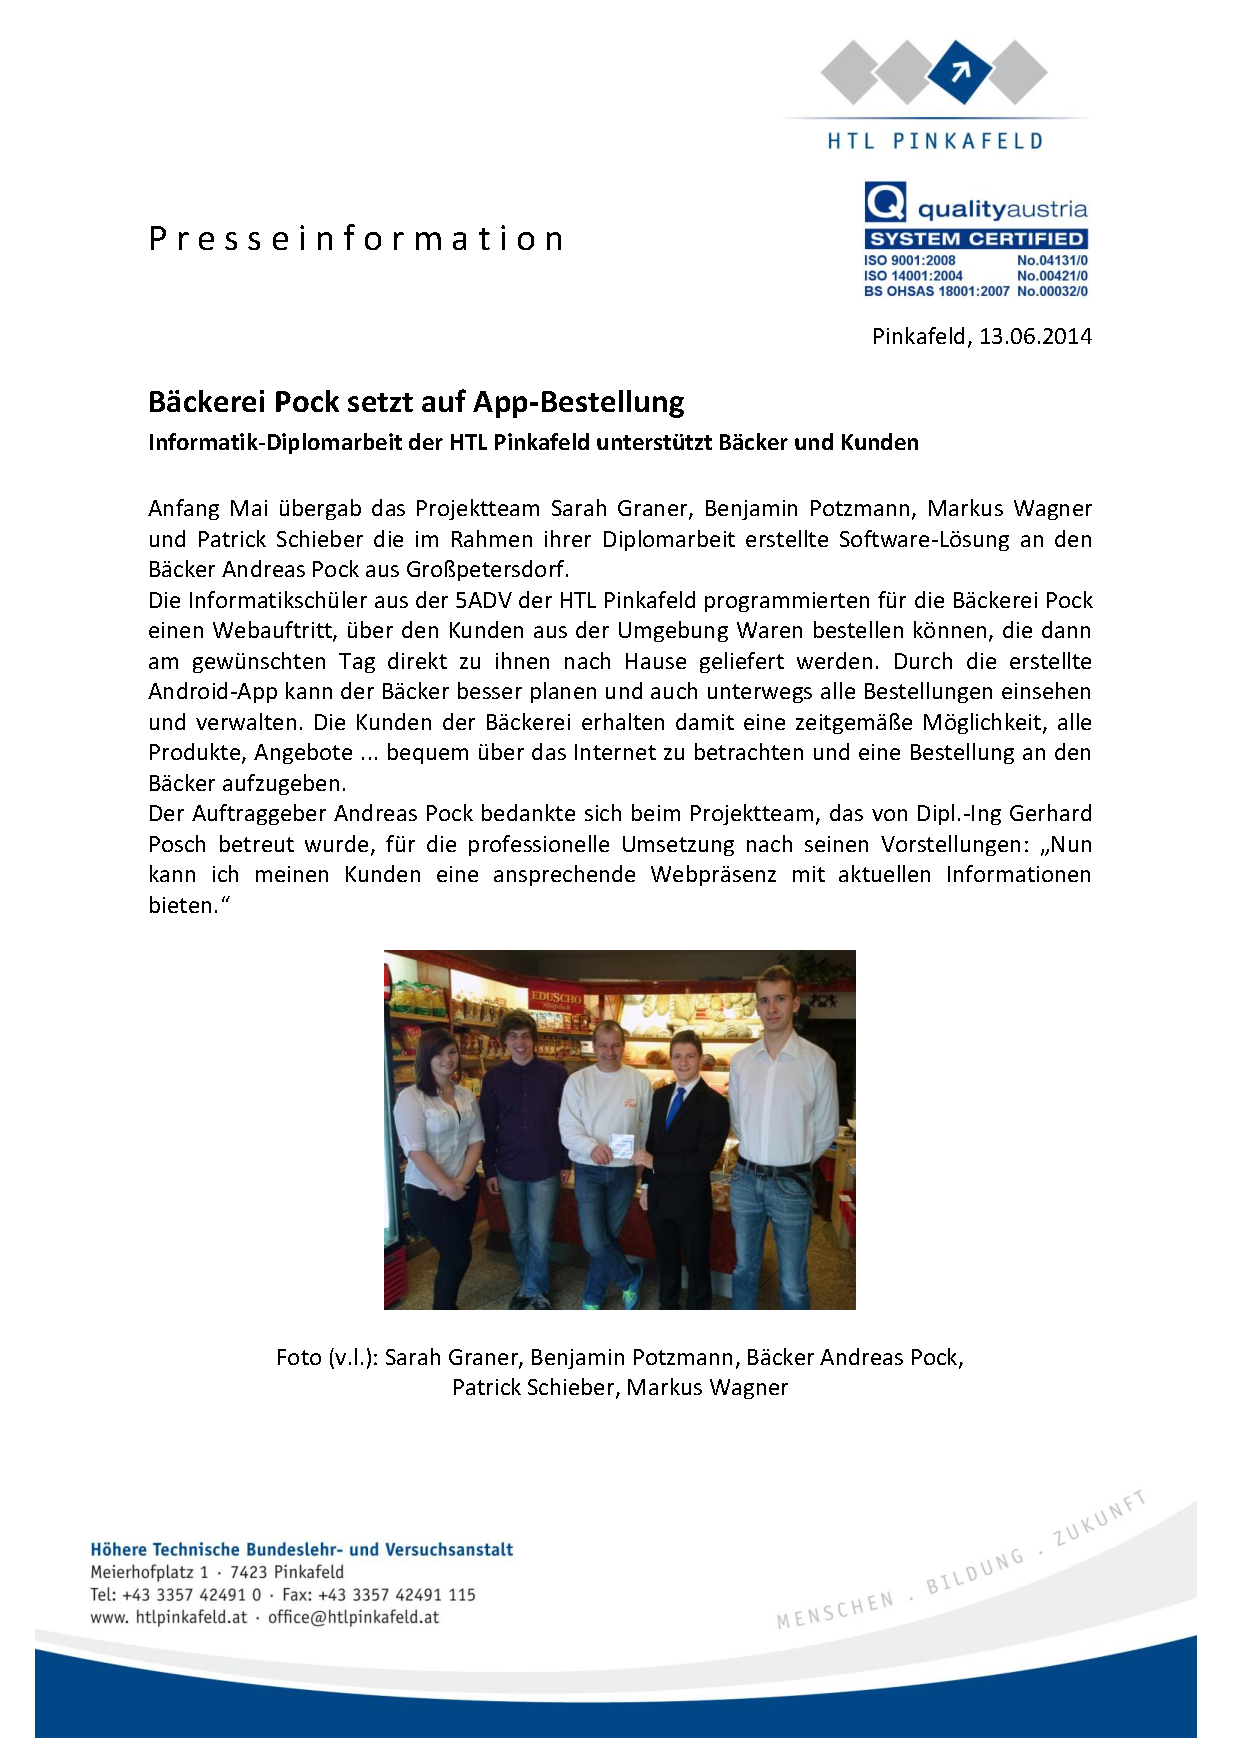
\includepdf[pagecommand={}]{figures/Beispiel.pdf}

% ohne:
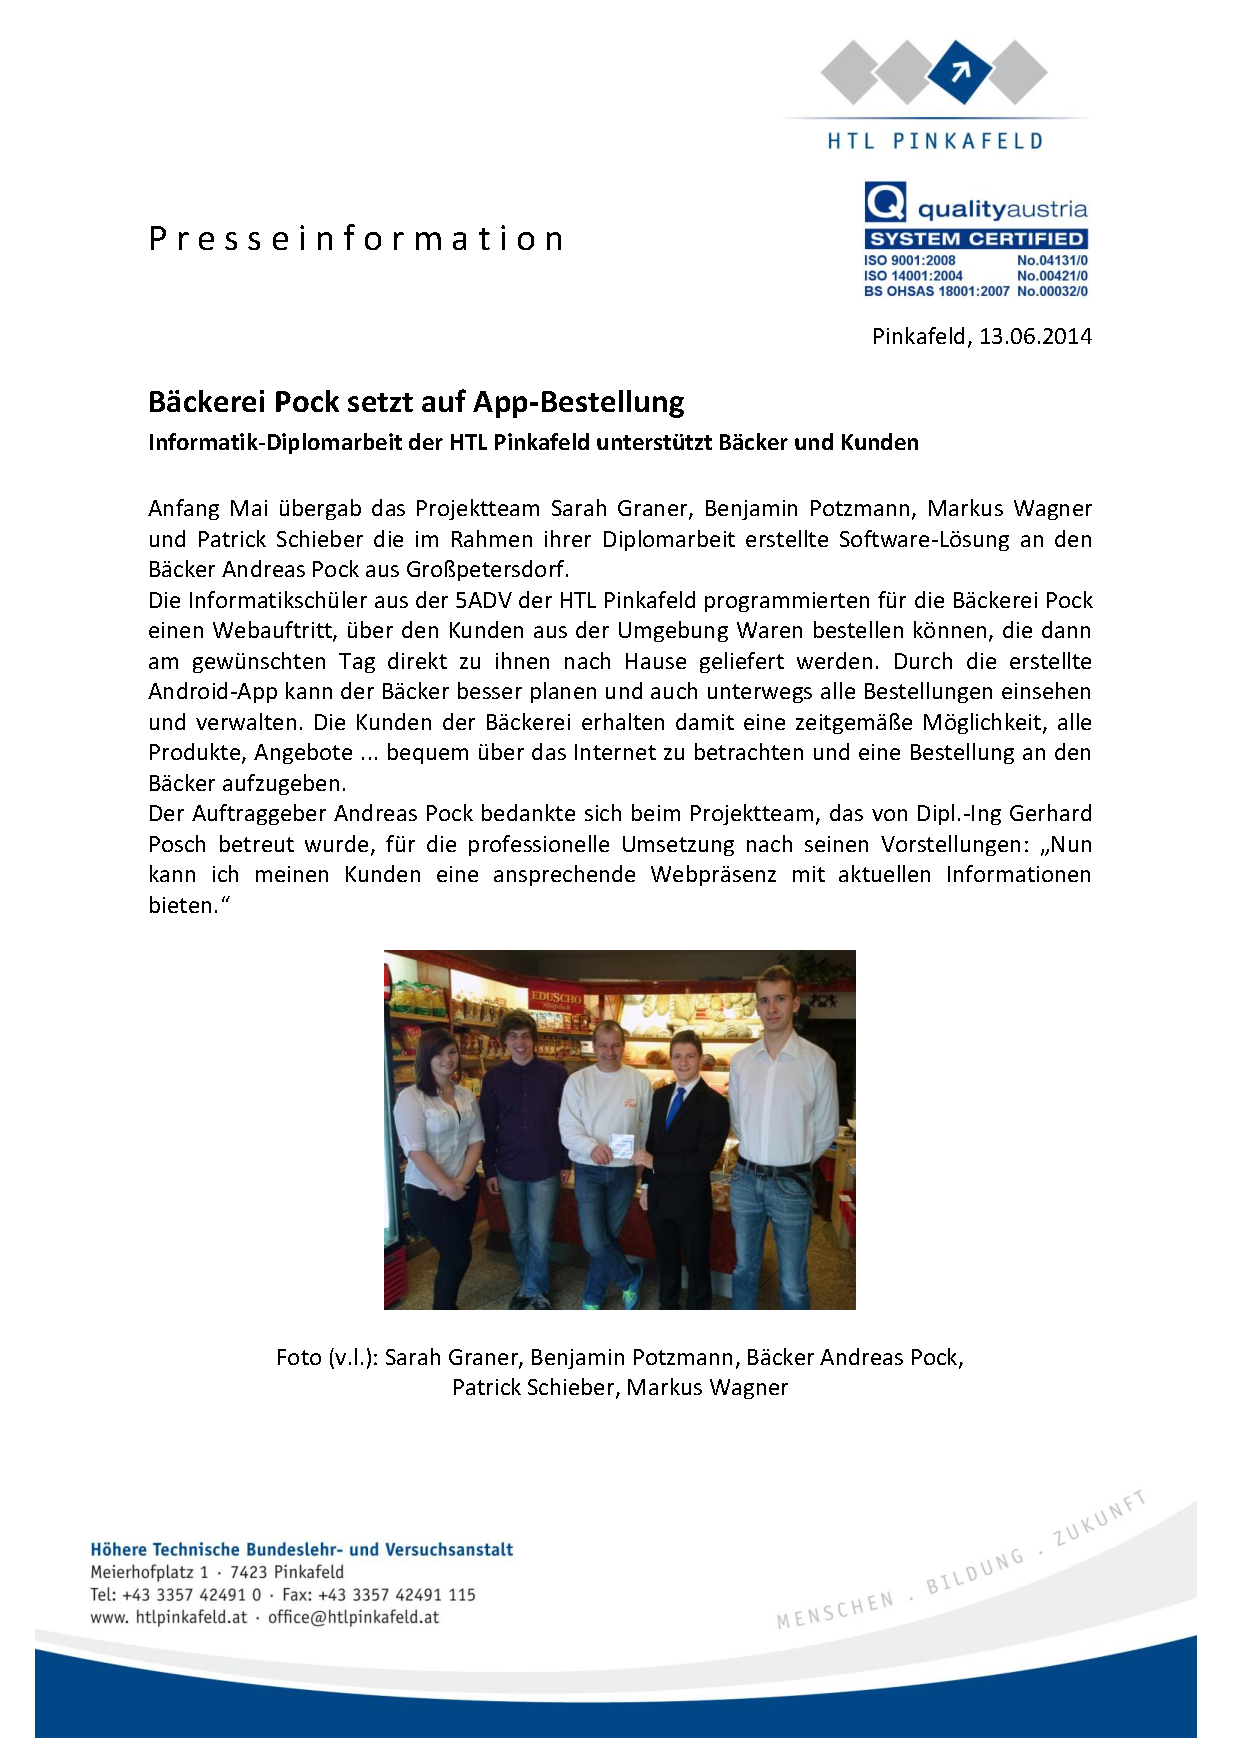
\includepdf{figures/Beispiel.pdf}

\end{document}

